\documentclass[Rapport/Rapport_main.tex]{subfiles}
\begin{document}
\section{RPi}
I dette segment af rapporten vil de væsentligste dele af RPiApp blive forklaret. Applikationen kan opdeles i tre dele: Et system til håndtering af trådsikret kommunikation og ressourcer, en Web applikation og en grafisk brugeroverflade. 
\subsection{RPiApp}
I dette afsnit fokuseres på softwarens 'event driven' arkitektur, trådkommunikation og logiske operationer - Alle klasser i systemet har en relation til GameController klassen i form af MsgQueue kommunikationen, men WebPage og Display anses som vigtige grænseflade klasser og får separate afsnit. 
En uddybende beskrivelse af klasserne kan findes i bilaget "Softwaredesign". 
\subsubsection{Softwaredesign}
\textbf{Event Driven Arkitektur:} \\
Beer Pong er et eventbaseret spil. Det omhandler masser af asynkrone handlinger; når der rammes ned i en kop, fjernelse af kop, indsættelse af mønt mm. Det er således utrolig vigtig, at vores system kan opfange alle disse asynkrone events. Selvom alle handlingerne fra brugeren er asynkrone, ønsker vi stadigt at interagere med handlingerne sekventielt. Dette er en vigtig faktor, da hvis en bruger laver to eventhandlinger inden for en kort tidsramme, skal vi sikre at systemet når at reagere på begge handlinger. En af måderne for at opnå dette er reaktiv programmering: Vi ønsker at opdatere vores system med det samme brugeren interagere med det. \\
Dette problem løses ved event driven arkitektur: Et system som reagerer ud fra signaler og tilstande fra aktører/delsystemer. Det er essentielt at de asynkrone signaler afvikles sekventiel og i et trådsikkert system. Her anvendes klassen MsgQueue, som er baseret på Producer / Consumer idiomet. 
\begin{figure}[H]
    \centering
    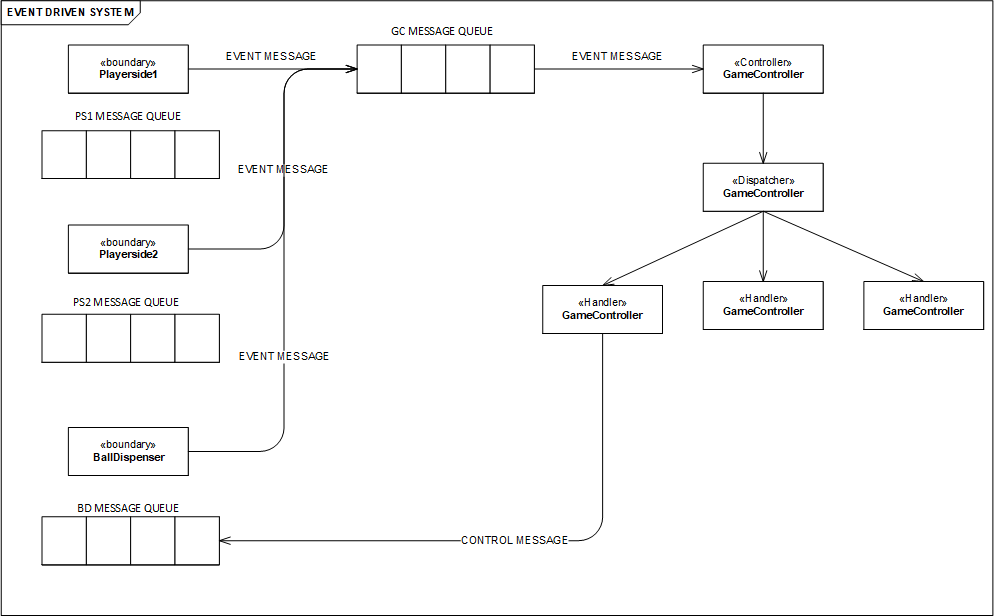
\includegraphics[width=1\textwidth]{Softwaredesign/RPiApp/graphic_RPi/EDS.png}
    \caption{Skitse af event driven system og MsgQueue system. Hvert boundary klasse har en MsgQueue instans, som er en 'consumer'. De andre klasser, som har tilgang til MsgQueue instansen, kan sende beskeder ved at allokerer besked. Beskeden består af et id og en instans nedarvet fra klassen 'Message'. Som det kan ses på skitsen, er der ingen klasser som har direkte 'kontakt' med hinanden, alt kommunikation sker gennem MsgQueues}
   \label{fig:Sketch_Event}
\end{figure}
MsgQueue-systemet indfører også et trådsikret system, da alt data sendt gennem MsgQueue instanserne er indkapslet af mutex'er. Desuden allokeres og deallokeres nedarvede beskeder af base klassen Message dynamisk - denne form for hukommelsesadministration sikre at ressourcerne bliver frigivet korrekt og der ikke opstår 'resource leaks'. For en mere detaljeret beskrivelse af event driven arkitektur, håndtering af ressourcer og design overvejelser, henvises til bilag "Software Design"\space afsnit \fullref{swdesign:sec:EventDriven}, samt afsnit \fullref{swdesign:sec:metode} for klassernes metodebeskrivelse.
\begin{figure}[H]
    \centering
    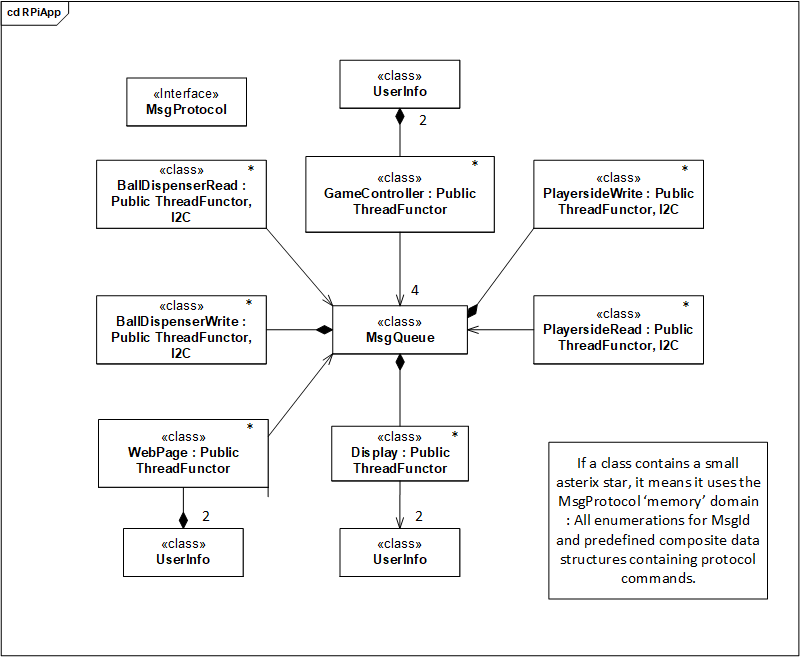
\includegraphics[width=1\textwidth]{Rapport/RPi/graphics/cd_RPiApp.png}
    \caption{Klasse diagram for RPiApp. Her ses det at alt kommunikation sker gennem MsgQueue - det kan derfor være svært at se klassernes relation til hinanden. MsgQueue og Message klasserne er udarbejdet i ISU undervisningen\autocite{MSGQUEUE}}
   \label{fig:cd_GameController}
\end{figure}
\textbf{RPiApp - GameController:}\\
Softwaredesignet for GameController, Playerside, BallDispenser, I2C og UserInfo er dokumenteret i afsnit X i bilaget "Softwaredesign". \\
Controller klassen, GameController, beskrives kort i dette afsnit, da den er essentiel for hele systemet. \\
RPiApp er omfangsrigt program og mange asynkrone handlinger og signaler skal behandles. GameController klassen er samlingspunktet for hele applikationen og indeholde alle de logiske operationer. Den bruger boundary klasserne til at dirigere PSoC-enhederne, WebPage og Display. 
\begin{figure}[H]
    \centering
    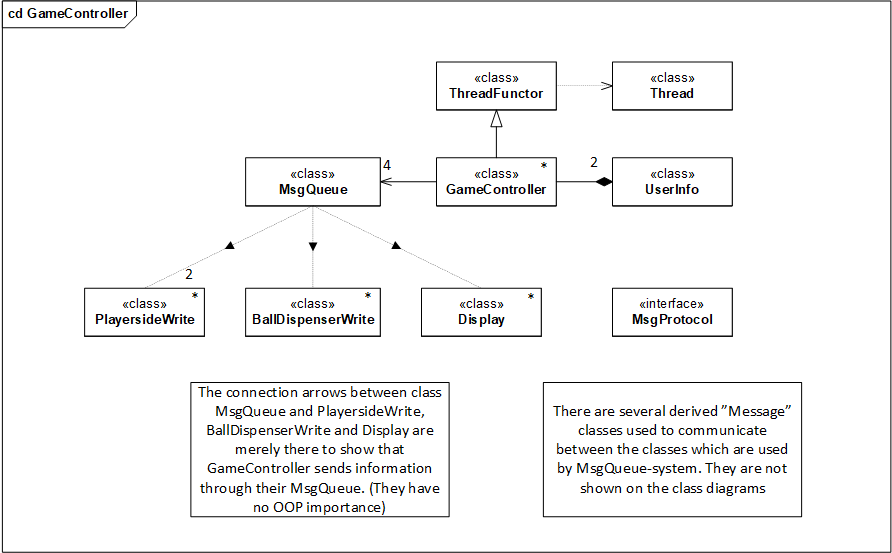
\includegraphics[width=1\textwidth]{Rapport/RPi/graphics/GameController.png}
    \caption{Klasse diagram for GameController. GameController anvender MsgQueue associationerne til at kommunikere med boundary klasserne. Boundary klasserne videreføre alle kommandoer udsendt fra GameController videre til delsystemerne som Playerside og BallDispenser enhederne}
   \label{fig:cd_GameController}
\end{figure}

\subsubsection{Implementering}
Softwareapplikation RPiApp er generelt udviklet objektorienteret i sproget C++17. Sproget bruges da det kan kompileres og afvikles på den valgte computerenhed, Rasberry Pi W Zero. C++ bruges til at udvikle det event driven arkitektur og det trådsikre system, men der bruges også elementer af C11 til at få adgang til filoperationer i Kernal Space.

RPiApp's kildekode kan findes i bilaget "Kildekode".

\subsubsection{Modultest}
Til test af GameController systemet blev white-box testing benyttet. Her blev de interne strukture testet, primært MsgQueue trådkommunikationen. Trådkommunikationen blev testet ved at sende dynamisk allokeret beskeder mellem klasserne, som indeholdt en MsgQueue (Producer / Consumer problemet). \\
Black-box testning blev også brugt til at teste grænsefladerne for de øvrige del-systemer: Playerside-enhederne og BallDispenser-enheden. Grænsefladen til begge enheder består af i2c kommunikation. Da det ikke er muligt at få adgang til Kernal Space operationer fra User Space, blev filoperationerne blot testet. \\\\
Begge tests er nærmere beskrevet i afsnittet \fullref{modultest:sec:test_Game} i bilaget "Modeltest"

\subsection{RPiApp - WebPage}
Dette afsnit omhandler boundary-klassen WebPage. I Beer Pong bordets RPi Zero W er der installeret en Apache web server, som er en populær webserver applikation, der gør det muligt at hoste hjemmesider.\cite{apache_web_server} Systemet giver brugerne mulighed for at tilgå hjemmesiden via smartphone, eller et andet mobilt device og indtaste holdnavne, brugernavne og holdfarve. WebPage er i denne forbindelse anvendt som en samlet betegnelse for alt, hvad der har med hjemmesiden at gøre. I virkeligheden består den af en klientside og en serverside, som kommunikerer internt gennem et WebSocket API. Den valgte løsning tager udgangspunkt i slides\cite{websockets_getting_started} fra en lektion med AU lektor S.Hansen. Der anvendes open-source biblioteket uwebsockets\cite{uwebsockets_repo} og visse elementer fra de eksempler, som blev præsenteret.

\subsubsection{Softwaredesign}
Et klassediagram for WebPage er vist i figur \ref{fig:WebPage_class_diagram}. For overskuelighedens skyld anvendes Client som betegnelse for den side, der vises i web browseren. Server anvendes som betegnelse for den C++ klasse, som skal modtage brugerdata fra Client og videreformidle disse til GameController klassen.
\begin{figure}[H]
    \centering
    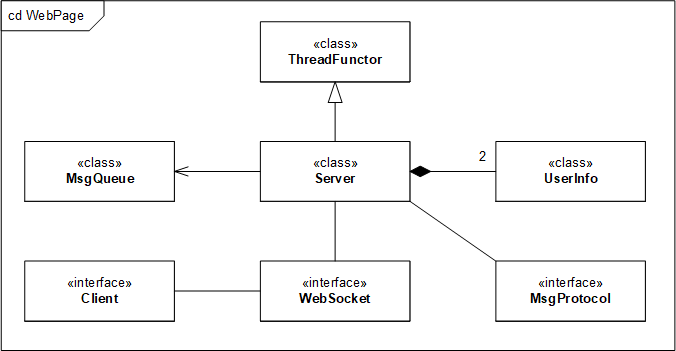
\includegraphics[width=1\textwidth]{Softwaredesign/RPiApp/graphic_RPi/cd_WebPage.png}
    \caption{Klassediagram for WebPage}
    \label{fig:WebPage_class_diagram}
\end{figure}

\\\\\textbf{Websocket}
\\Web kommunikation forløber typisk ved, at der etableres et forhold mellem client og server, som er baseret på anmodninger og svar. Client kan eksempelvis være en web browser og server en applikation, som hoster en hjemmeside. En ofte anvendt protokol til denne form for kommunikation er HTTP.\cite{http_wiki} HTTP er en request-response protokol, og kommunikationen er som regel initieret af client. Client sender en HTTP request eller besked til serveren, og server svarer igen med et HTTP response, som både kan indeholde status information, eller andet indhold, der er anmodet om. \\Ved at opdatere HTTP forbindelsen til en WebSocket kan der etableres en vedvarende forbindelse mellem client og server. Kommunikationen kan betegnes som full-duplex og graden af overhead er sænket.\cite{websocket_wiki} Der oprettes et egentligt WebSocket objekt og events samt metoder, som er associeret med dette objekt er beskrevet nærmere i dokumentet Softwaredesign i afsnit \fullref{swdesign:sec:websocket_doc}.

\\\\\textbf{Client}
\\Client beskriver hjemmesidens interface. Det er her defineret, hvordan hjemmesiden skal præsentere sig i web browseren. Under initieringen af siden oprettes WebSocket objektet, og de event handlers som er en del af API er ligeledes implementeret her. Når data skal sendes mellem Client og Server skal det ske i tekstformat. Der er derfor designet en løsning, hvor spillerne har mulighed for at indtaste holdnavne og brugernavne samt vælge holdfarver på track bars for henholdsvis hold 1 og hold 2. Når der trykkes på en 'Start' knap på hjemmesiden genereres et event, som medfører, at alle brugerinputs konkateneres til én tekststreng og sendes til serveren. Denne fremgangsmåde virker efter hensigten i vores tilfælde, da hjemmesiden skal behandle relativt få inputs. Med mange inputs kan den godt resultere i komplicerede operationer, da tekststrengen skal splittes ad igen og konverteres til det rette format. Alternativt kunne man have opbevaret data i et JavaScript objekt og konverteret dette til JSON.\cite{json_intro} JSON er tekst, og på denne måde kunne større mængder af data sendes mellem Client og Server uden de komplicerede operationer for at splitte og oversætte det.

\\\\\textbf{Server}
\\Serversiden har til opgave at modtage og behandle førnævnte data fra client og er implementeret som en C++ klasse. Den lytter aktivt på den relevante port, og når tekststrengen modtages bliver denne indlæst i en buffer og separaret på passende vis. Informationerne opbevares i en STL container og anvendes til at sætte members på to objekter af UserInfo klassen, team1\_ og team2\_. Disse objekter skal sendes til GameController klassen, og hertil anvendes det tidligere beskrevne event drevne system med Messages og MsgQueues. WebPage har derfor kendskab til GameControllers MsgQueue, men det omvendte gør sig ikke gældende. Hvis GameController først sendte en request besked for herefter at modtage objekterne i en responsebesked fra server kunne der hurtigt opstå komplikationer. Der blev forudset problemer med race conditions og problematisk adfærd. Kommunikationen mellem server og GameController er derfor bevidst gjort envejs så dette undgås, og dermed sikres det også, at GameController altid arbejder på de nyeste brugerinputs. Da kommunikationen er gjort envejs, kan det diskuteres, om der er behov for den full-duplex kommunikation, som et WebSocket API tilbyder. Designet er imidlertid baseret på en forestilling om, at det var GameController, som i det rigtige stadie af spillet skulle sende en request om data. Kommunikationen ville da blive initieret af server og der ville være behov for en løsning som f.eks. et WebSocket API. Som resultat af den iterative udviklingsproces måtte WebSocket designet genovervejes, men det var ikke nødvendigt at ændre designet, selv om kommunikationen blev forsimplet.\\\\WebPage er forsøgt opsummeret i et sekvensdiagram i figur \ref{fig:WebPage_sequence_diagram}. Det viser, at brugeren interagerer med client, når der skal indtastes holdoplysninger, mens Client og Server kommunikerer gennem et WebSocket API, som tidligere beskrevet. Serveren benytter sig af klassen UserInfo og sender to objekter af denne til GameControllers MsgQueue.  
\begin{figure}[H]
    \centering
    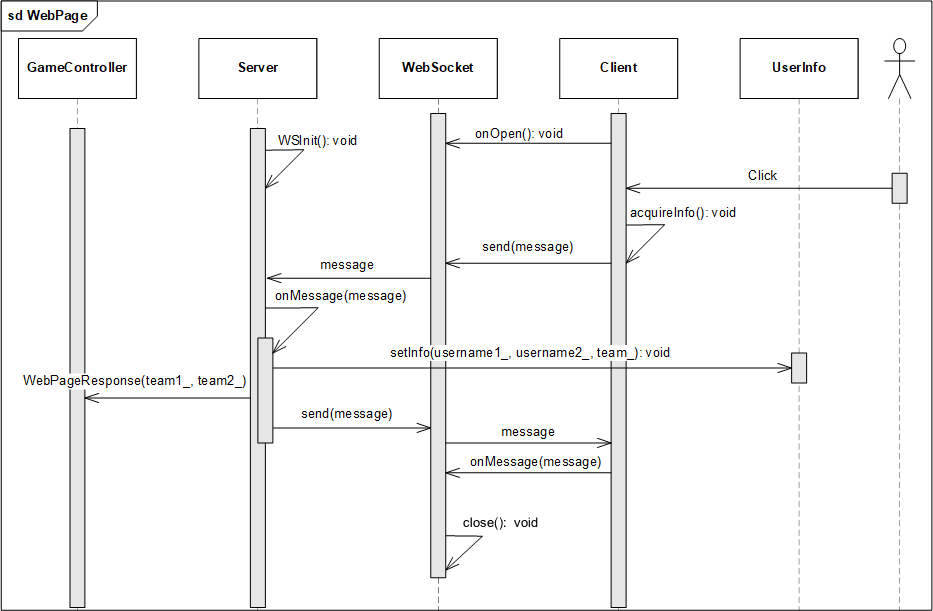
\includegraphics[width=1\textwidth]{Softwaredesign/RPiApp/graphic_RPi/WebPage_sd_2.png}
    \caption{Sekvensdiagram for WebPage}
    \label{fig:WebPage_sequence_diagram}
\end{figure}
\subsubsection{Implementering}
Webserver hostes som bekendt af en RPi Zero W. Den er derfor implementeret som en C++ klasse i sproget C++17. Hjemmesidens interface beskrevet i afsnittet \textbf{Client} er implementeret med det såkaldte 'markup language' HTML5 i kombination med Cascading Style Sheets (CSS). Script-sproget Javascript anvendes til at implementere hjemmesidens dynamiske elementer samt WebSocket API. For flere informationer vedrørende implementeringen henvises til dokumentet Softwaredesign i afsnittet \fullref{swdesign:sec:webpage_implementering}

\subsubsection{Modultest}
De vigtigste krav for WebPage er opsummeret  nedenfor.
\begin{itemize}
    \item Alt tekst på WebPage skal være på sproget engelsk
    \item På WebPage skal der for hvert af de to hold indtastes følgende \textit{\textbf{spiller oplysninger}}: \textit{teamname}, \textit{username1} og \textit{username2}
    \item Holdnavne og brugernavne indtastet på WebPage skal være tekststrenge, med en længde på mellem 1 og 15 karakterer
    \item På WebPage skal der for hvert af de to hold kunne vælges følgende \textit{\textbf{spiller oplysninger:}} \textit{holdfarve}, ved at justere intensiteten af farverne rød, grøn og blå i et RGB farveskema.
    \item Der skal kunne vælges mindst 10 forskellige farver på WebPage.
\end{itemize}
For at teste kravene er der lavet et testprogram, som udskriver \textit{\textbf{spiller oplysninger}} i terminalen i ubuntu, hver gang data sendes fra Client til Server. Testen foretages ved at indtaste \textit{\textbf{spiller oplysninger}} på hjemmesiden, trykke 'Start' og herefter undersøge terminal output. Dette gentages 50 gange, mens navne og farver varieres, og resultatet fremgår af tabellen nedenfor.
\begin{table}[H]
    \centering
    \begin{tabular}{|L{0.15\textwidth}|L{0.15\textwidth}|L{0.15\textwidth}|}
         \hline
         \textbf{Forsøg, n} & \textbf{Korrekt output} & \textbf{Fejl} \\ \hline
         50 & 50 & 0 \\ \hline 
    \end{tabular}
    \caption{Data sendes fra client til server 50 gange}
     \label{tab:webpage_data_2}
\end{table}
Hjemmesiden er vist i browseren i figur \ref{fig:webpage_modultest_rapport_1}, mens det resulterende terminal output fremgår af figur \ref{fig:webpage_modultest_rapport_2}.
\begin{figure}[H]
    \centering
    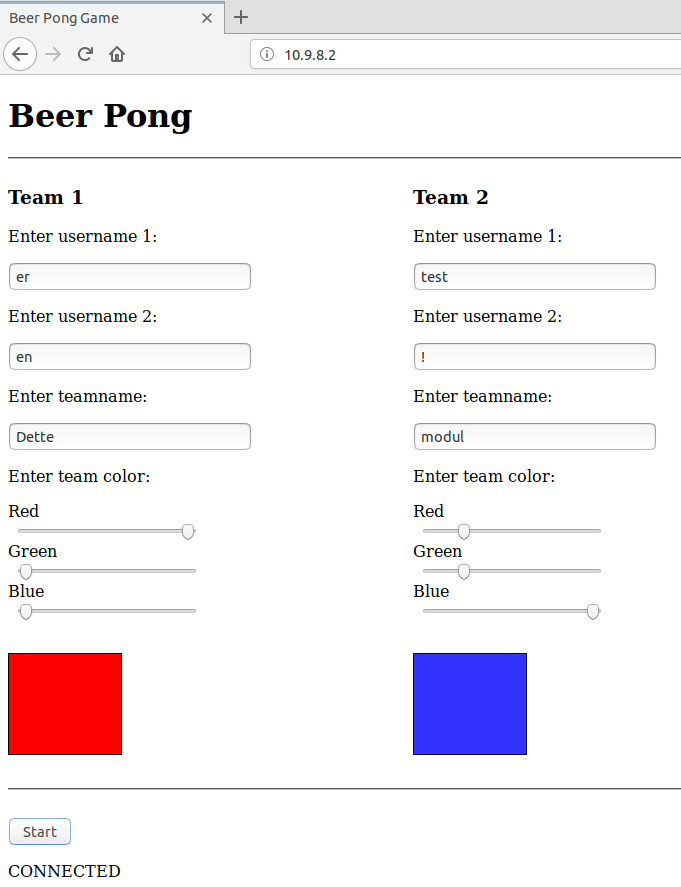
\includegraphics[width=0.6\textwidth]{Modultest/WebPage/graphics/modultest_1.png}
    \caption{Modultest - hjemmeside vist i browser}
    \label{fig:webpage_modultest_rapport_1}
\end{figure}
\begin{figure}[H]
    \centering
    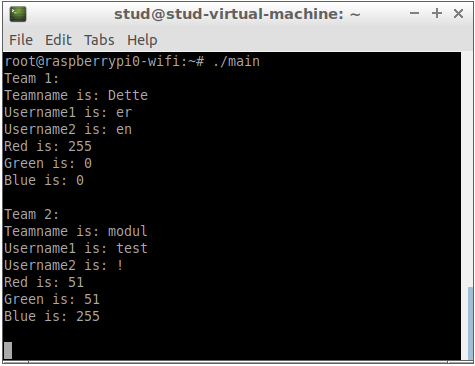
\includegraphics[width=0.5\textwidth]{Modultest/WebPage/graphics/modultest_2.png}
    \caption{Modultest - terminal output}
    \label{fig:webpage_modultest_rapport_2}
\end{figure}
Ved visuel inspektion af hjemmesiden i figur \ref{fig:webpage_modultest_rapport_1} kan det konkluderes, at kravene angivet ovenfor er opfyldt. Desuden virker det til, at \textit{\textbf{spiller oplysninger}} sendes korrekt fra Client til Server. For yderligere informationer vedrørende modultesten henvises til dokumentet Modultest i afsnittet \fullref{modultest:sec:webpage_modultest}

\subsection{I2C\_interruptDriver}
\subfile{Rapport/RPi/I2C_interruptDriver/Design.tex}
\subfile{Rapport/RPi/I2C_interruptDriver/Implementering.tex}
\subfile{Rapport/RPi/I2C_interruptDriver/Modultest.tex}

\subsection{RPiApp - GUI}
\subsubsection{Softwaredesign}
\subfile{Softwaredesign/GUI/GUI_software_rapport.tex}
\subsubsection{Implementering}
\subfile{Softwaredesign/GUI/GUI_implementering_rapport.tex}
\subsubsection{Modultest}



\end{document}